\chapter{Evaluation}
\label{chap:evaluation}
% "Moreover, under large record size (e.g., 1KB and above), B+ tree tend to have smaller write amplification than LSM-tree." - from "Closing the B+-Tree vs. LSM-Tree Write Amplification Gap on Modern Storage Hardware with Built-in Transparent Compression", Qiao et al., FAST 2022
% Good evaluation paper: https://dl.acm.org/doi/pdf/10.1145/3183713.3196895
% To adhere to the DAM model, can't we assume that all inner nodes are cached in memory, but leafs are not? see "A Comparison of Fractal Trees to Log-Structured Merge (LSM) Trees"

% Observations:
% We erase a lot of entries in the Delta Tree, which causes a lot of fragmentation and caused significantly more nodes.
% - The higher the fanout of the tree, the higher the write amplification we introduce in the Delta Tree itself.
% - We essentially amplified the write amplification in the system.
% WA becomes worse the bigger the Delta Tree becomes in relation to the Base Tree.
% - When we compacitified after every erase, we saw a reduction in write amplification again.
% - Now we reduce write amplification for small threshold (5-10%), but increase it for higher thresholds (20-50%).

% - We reduce write amplification only if we write out a Delta Tree node with more than one entry since the last write-out.
% - If we always write out a Delta Tree node already after a single change, we do not benefit.
% - We should see that effect when our buffer is too small and we cannot cache anything.
% - Buffering only makes sense if we can cache changes.

% - Everytime we load a B-Tree node, we perform a lookup into the Delta Tree.

% Mention that we do not take into accound construction and destruction of the index, since we are interested in steady state performance.

\section{Experimental Setup}
Since we are interested in write amplification, we observe the number of page writes to disk for different workloads and different memory limitations.
This way, our results are not biased by the specific implementation, optimizations, and hardware that we run our experiments on.
All experiments were conducted locally on a Apple MacBook Pro with the specification listed in \autoref{tab:hardware-specs}.

\begin{table}[htbp]
\centering
\caption{Hardware Specifications}
\label{tab:hardware-specs}
\begin{tabular}{ll}
\toprule
\textbf{Component} & \textbf{Specification} \\ 
\midrule
Device & Apple MacBook Pro (2021) \\
Processor (CPU) & Apple M1 Pro (8-core, up to 3.2\,GHz) \\
GPU & Integrated 14-core Apple GPU \\
Memory (RAM) & 16\,GB \\
Storage & 512\,GB NVMe SSD \\
Operating System & macOS Sonoma 14.6.1 \\
\bottomrule
\end{tabular}
\end{table}

\section{Workloads and Datasets}
We evaluate our approach on synthetic and real-world datasets.
The real-world dataset allows us to evaluate our approach on realistic data distributions and access patterns.
With the synthetic dataset, we can control the data distribution to evaluate the performance of our approach under different scenarios.
This allows us to identify the strengths and weaknesses of our approach.

We will be evaluating our system as a whole, benchmarking the database with the different indices to gain a holistic view of the performance.
To take a closer look at the indices themselves, we will also be benchmarking the indices in isolation, without the overhead of the database system.
For example, when benchmarking the whole database, we have to maintain the table data as well as the index, which introduces additional overhead.
When benchmarking the index in isolation, we can focus on the performance of the index itself.

\subsection*{Wikipedia Pageviews Workload}
We use an augmented Wikipedia Pageviews dataset \cite{wiki_pageviews} as a real-world dataset for our evaluation.
The primary goal of this dataset is to evaluate the performance of our approach on realistic data distributions and access patterns.
The dataset contains pageview statistics for all Wikipedia articles within a certain time frame.
It is publicly available and can be downloaded from the Wikimedia Dumps website\footnote{https://dumps.wikimedia.org/other/pageviews/}.
Each pageview record is of the form 
$$
\texttt{en Google\_Chrome 10406 0}
$$
consisting of the domain code, the page title, the number of views, and  the total response size in bytes.

\subsubsection*{Data Augmentation}
We use the hourly Pageview Wikipedia dataset from 1st of October 2025 at 00:00 UTC as our base dataset.
We augment the dataset in the following way:
\begin{enumerate}
    \item We filter out all non-English articles, i.e., we only keep articles with the domain code \texttt{en}.
    \item For benchmarks with integer keys, we turn the page title into an integer key. For benchmarks with variable-sized keys, we use the original page title as key.
    \item We create a lookup operation for each view of an article, i.e., if an article has 100 views, we create 100 lookups for that article.
    % TODO: update the actual percentage we used.
    \item To generate a mixed workload, we turn a certain percentage of the lookups into updates. This assumes that an article with more views is more likely to be updated.
    \item We then shuffle the operations to create a mixed workload.
    % TODO: update the percentage of the sample we used.
    \item To create a smaller dataset, we take a random fraction of the articles as samples.
\end{enumerate}

To populate the database, we insert all articles from filtered dataset once.
We then run the workload on the database or on the indices directly.

\subsubsection*{Workload Characteristics}
\label{sec:workload-characteristics}
The resulting workload has the following characteristics:
\begin{itemize}
    \item The dataset contains 59,240 distinct articles, translating to 59,240 distinct keys in the database.
    \item The workload contains 146,068 views in total.
    \item The keys follow a Zipf-like distribution, i.e. a small number articles are very popular and receive a large number of operations, while the majority of articles receive only a few. 
    \item In fact, 40,670 articles (\textasciitilde69\%) are viewed only once in the dataset. 
    The most viewed article, \textit{Jon\_Stewart}, received 2,998 views (\textasciitilde10\% of all views).
    \item \textbf{Update workload}: We transform 7,303 lookups into updates (\textasciitilde5\%) by default. When mentioned, we vary the update ratio from 0\% to 100\%.
    \item With an update ratio of 5\%, we update 5,724 distinct articles (\textasciitilde10\% of all articles) in the generated workload, whereas the majority of articles (\textasciitilde86\%) are only updated once.
    The most frequently updated article, \textit{Jon\_Stewart}, is updated 132 times (\textasciitilde10\% of all updates).
    \item \textbf{Insert workload}: To evaluate the performance of our approach on insert-heavy workloads, we create a workload with 100\% inserts as well.
    In this workload we insert all articles of the sample into an empty database or index.
    \item The keys are variable-sized strings with an average length of 20.5 characters, a maximum length of 236 characters and a minimum length of 1 character.
\end{itemize}

\section{Results and Analysis}
In this section, we present the results of our benchmark experiments and analyze the performance of the B-Tree and BBB-Tree indices.
Our primary metric for this evaluation is the number of page writes to disk, which we aim to reduce.
We also analyze the space overhead and read amplification introduced by our approach.

The goal of this evaluation is to determine whether the BBB-Tree can reduce page writes compared to a traditional B-Tree under different workloads and memory constraints.
Additionally, we want to understand the trade-offs involved in using a BBB-Tree.

\subsection{Write Amplification}
For a first analysis, we consider the write amplification of the B-Tree and BBB-Tree indices when running the mixed Wikipedia Pageviews workload on the database.
We run the workload with 4 KB pages, a buffer pool of 500 pages, and a write threshold of 5\% (i.e. we only write pages to disk if at least 5\% of the page has been modified in the case of a BBB-Tree index).
We compare the number of page writes to disk for both indices.
To gain a holistic view of the performance, we run the workload on the database as well as on the indices directly.
The results are shown in \autoref{fig:both}.
When running the workload on the database as a whole (\autoref{fig:sub1}), we see a reduction in page writes of \textasciitilde23\% when using the BBB-Tree compared to the B-Tree.
When running the workload on the indices directly (\autoref{fig:sub2}), we see a more significant reduction in page writes of \textasciitilde66\% when using the BBB-Tree compared to the B-Tree.

There are two main reasons for the difference in write amplification reduction between the two scenarios.
\begin{enumerate}
  \item \textbf{Relative Impact}: Firstly and more obviously, when running the workload on the database, we have more pages in the system that are not affected by our method.
Our method effects a smaller fraction of the total number of pages in the buffer, therefore our relative impact is naturally smaller.
When running the workload on the indices directly, we can focus on the performance of the method itself without the overhead of maintaining the table data.
Therefore, we will focus on the results when running the workload on the indices in isolation in the following analysis.
  \item \textbf{Memory Constraints}: More importantly, the indices have different memory constraints in the two scenarios.
When running the workload on the database, the indices have to share the buffer pool with the table data.
When running isolated, the indices can use the full memory available in the system. 
In the metrics collected during the benchmark runs, we could see that we have 10-15\% higher buffer hit rates when running the workload on the indices directly.
While both indices have the same memory available and higher buffer hit rates when running isolated, the BBB-Tree performs better in terms of write amplification reduction.
\end{enumerate}

These findings indicate that the BBB-Tree can significantly reduce write amplification compared to a traditional B-Tree, especially when the index can effectively utilize the available memory.
To investigate this further, we will run the workload under different memory constraints in the following section.

\begin{figure}[htbp]
  \centering
  \begin{subfigure}[b]{0.49\textwidth}
    \centering
    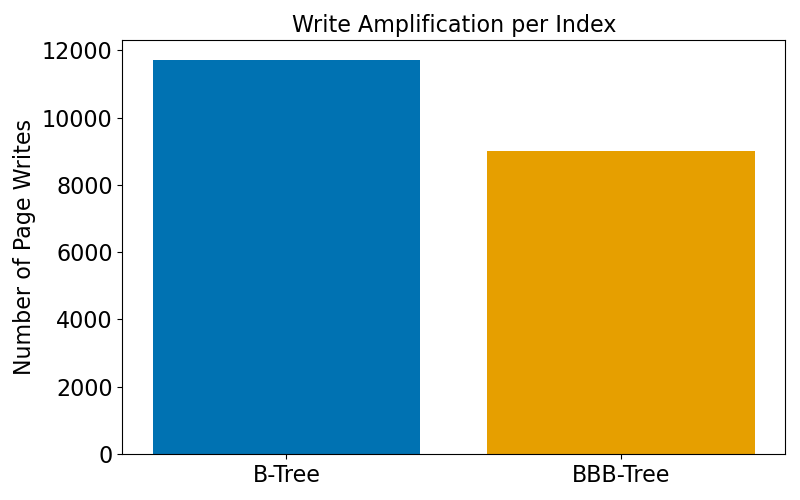
\includegraphics[width=\textwidth]{figures/evaluation/pageviews_mixed_db.png}
    \caption{Running the workload on the database with different indices.}
    \label{fig:sub1}
  \end{subfigure}
  \hfill
  \begin{subfigure}[b]{0.49\textwidth}
    \centering
    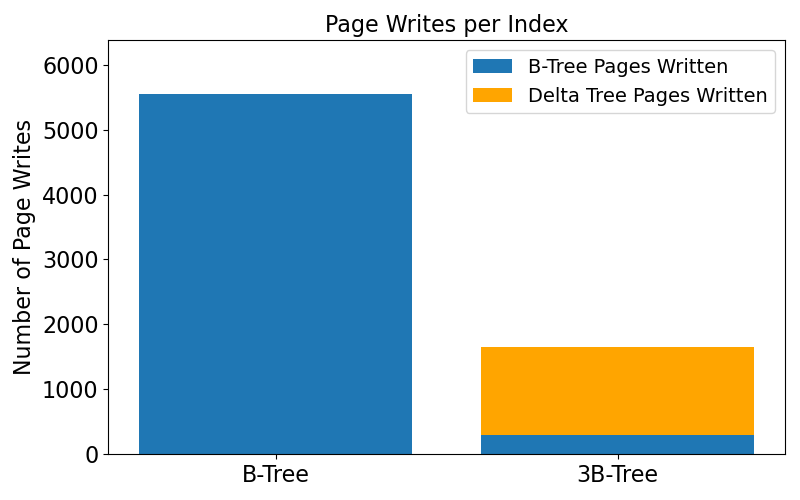
\includegraphics[width=\textwidth]{figures/evaluation/pageviews_mixed_index.png}
    \caption{Running the workload on the indices directly.}
    \label{fig:sub2}
  \end{subfigure}
  \caption{Running the mixed Wikipedia Pageviews workload with 5\% updates, 4 KB pages, a buffer pool of 500 pages, and a write threshold of 5\%. We see a significant difference in write amplification reduction when running the index as part of the database vs. running it in isolation.}
  \label{fig:both}
\end{figure}

\subsubsection*{Different Memory Constraints}
To understand the impact of memory constraints on the performance of the BBB-Tree, we run the same workload with different buffer pool sizes.
The workload produces a B-Tree of 606 nodes in total. We vary the buffer pool size from 50 to 700 pages, while keeping the page size at 4 KB.
The results are shown in \autoref{fig:buffer_sizes}.

\begin{figure}[htbp]
  \centering
  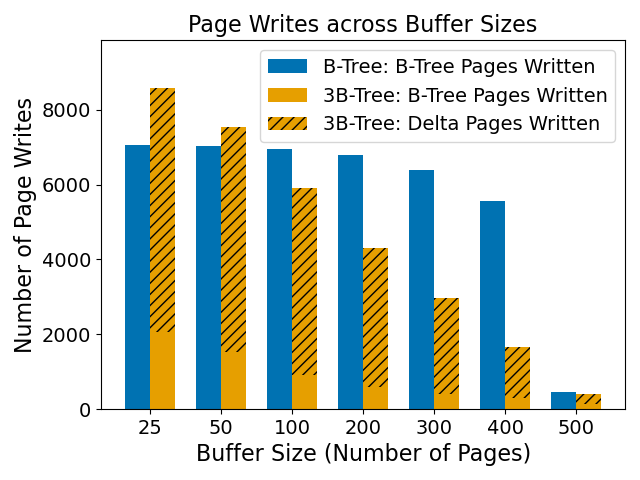
\includegraphics[width=0.7\textwidth]{figures/evaluation/pageviews_buffer_sizes.png}
  \caption{The impact of buffer pool size on the amount of page writes per index with a 4 KB page size and a 5\% write threshold. The BBB-Tree performs better with higher buffer pool sizes, as it can accumulate more changes in memory before writing them to disk. When the buffer fits the whole index, we perform no page writes at all.}
  \label{fig:buffer_sizes}
\end{figure}

\inlinesection{Low Memory Capacity.}
With a buffer pool of 50 to 100 pages, we have little memory to cache changes.
The BBB-Tree suffers from the limited memory more than the B-Tree and we even see an increase in page writes.
This is, because with every load and eviction of a B-Tree page, we we have to perform operations on the Delta Tree, loading additional pages into memory.
This reduces the chances of caching any updates in memory.
Our method aims to only introduce overhead to the point in time of B-Tree page swaps.
If we constantly swap pages in and out of the buffer pool to perform any operation, we introduce more overhead.

For example, consider two temporally close updates to the same B-Tree node. 
The traditional B-Tree has a higher chance to batch these updates into a single page write.
With the BBB-Tree however, the first updates is more likely to be written to disk before the second update arrives, leading to two page writes instead of one.
With very limited memory, we amplify the write amplification in the system.

Let us assume we do not cache any pages in memory, we only hold those pages that we need to perform the current operation and evict them immediately afterwards.
Given a B-Tree of height $h$ and a Delta Tree of height $d$, we can analyze the memory requirements for updating a leaf node in the B-Tree.
To update a leaf node in the B-Tree, we have to fix $h$ pages in memory (one for each level of the tree).
For every node that we load from disk, we have to check the Delta Tree for any updates to apply.
This means that we need a total of $h * d$ pages loads to perform an update.
This is a worst case scenario that we approach when we have very limited memory.
If we have a B-Tree of height 3 and a Delta Tree of height 2, we need to load $3 * 2 = 6$ pages to perform any operation on the B-Tree.
With a sufficient amount of memory, we can assume that inner nodes are already in memory, reducing the number of page loads to $1 + 1 = 2$.
As soon as we have enough space to cache pages effectively, we can start to accumulate changes in memory and reduce page writes.

This makes one trade-off of our method very clear:
We sacrifice some space in memory to cache and batch changes.
This means that we have less memory available to cache B-Tree pages.
Therefore, we need to swap B-Tree pages more often, leading to more page writes.
Only with the ability to hold changes in memory long enough to batch them, we can reduce the page writes in total.
In a very low memory setting, we introduce more page writes than we save.

\inlinesection{Full Memory Capacity.}
When the buffer pool can hold the whole B-Tree (700 pages), we perform no page writes at all with the BBB-Tree, as all changes can be accumulated in memory.
In this scenario, the Delta Tree remains empty and the BBB-Tree is obsolete.
However, we noticed in our benchmarks that the BBB-Tree does not introduce significant overhead when the whole index fits in memory.
When initially loading pages into memory, we have to perform one lookup into the empty Delta Tree for each B-Tree node.
However, once the buffer cache is hot and all pages are loaded into memory, we do not have to perform any additional operations on the Delta Tree, as all changes can be applied directly to the B-Tree nodes in memory.
The only overhead that remains is tracking the changes to the B-Tree nodes.
In the benchmarks, we see that the BBB-Tree is \textasciitilde0.67\% slower than the B-Tree in this scenario.

\inlinesection{Restricted Memory Capacity.}
With reasonably limited memory capacities (200-600 pages), we see a significant reduction in page writes with the BBB-Tree compared to the B-Tree.
With a buffer pool of 500 pages, we see a reduction in page writes of \textasciitilde66\% with the BBB-Tree compared to the B-Tree.
The larger the available memory, the more changes we can accumulate in our Delta Tree before writing them to disk.
We achieve the batching effect that we are aiming for, leading to fewer page writes.
This shows that our method can effectively utilize the available memory to reduce write amplification in memory-constrained settings.
We require about 1/4 of the index fit in memory to see significant improvements and it defers page writes best when 2/3 of the index fit in memory.

\inlinesection{Summary.}
To summarize, the BBB-Tree aims to reduce write amplification in memory-constrained settings where the entire dataset cannot fit in memory.
Its efficiency depends on caching mechanisms that group updates into fewer page writes. 
This optimization is achievable only when enough memory is available for effective caching.

\subsubsection*{Different Write Thresholds}
To understand the impact of the write threshold on the performance of the BBB-Tree, we run the same workload with different write thresholds.
We fixate the buffer pool size at 500 pages and the page size at 4 KB.
To repeat, the write threshold defines the minimum percentage of a page that has to be modified before we write it to disk.
When it is smaller than the threshold, we accumulate the changes in the Delta Tree and defer the write.
For the baseline B-Tree, the write threshold has no effect, as we always write every change to disk immediately.
We vary the write threshold from 0\% to 100\%.
The results are shown in \autoref{fig:write_thresholds_improvement}.

\begin{figure}[ht]
  \centering
  \begin{minipage}{0.48\textwidth}
    \centering
    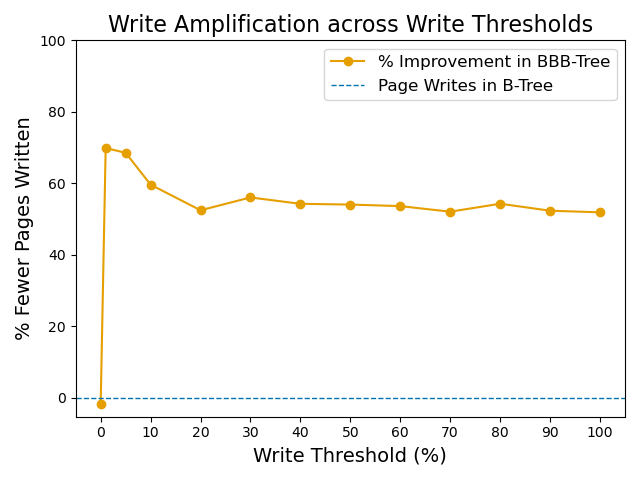
\includegraphics[width=\textwidth]{figures/evaluation/pageviews_write_thresholds_improvement.png}
    \caption*{(a) Workload: 5\% updates \& 95\% lookups. Buffer Size: 500 pages. Page Size: 4 KB.}
  \end{minipage}\hfill
  \begin{minipage}{0.48\textwidth}
    \centering
  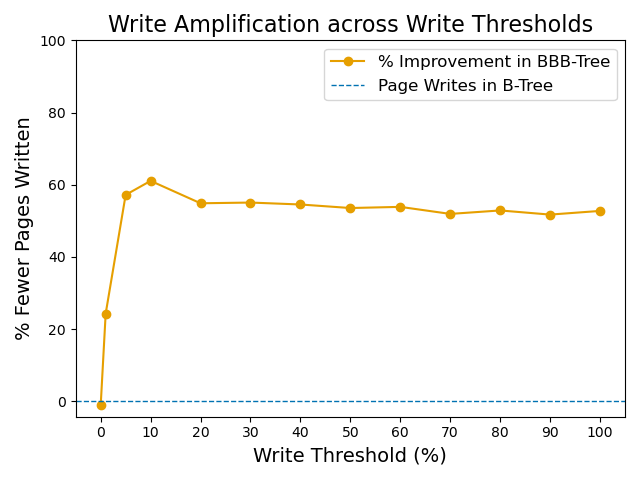
\includegraphics[width=\textwidth]{figures/evaluation/pageviews_write_thresholds_improvement_inserts.png}
    \caption*{(b) Workload: 100\% inserts. Buffer Size: 300 pages. Page Size: 4 KB.}
  \end{minipage}
  \caption{The impact of different write thresholds on the amount of page writes per index on two different workloads. At 0\% threshold, we write every B-Tree node to disk after every change, leading to no improvement in write amplification. With higher thresholds, we can accumulate changes before writing them to disk, leading to significantly fewer page writes. Both workloads show similar trends, with the BBB-Tree performing best with small write thresholds.}
  \label{fig:write_thresholds_improvement}
\end{figure}

\inlinesection{Without Buffering.}
With a write threshold of 0\%, we write every changed page to disk immediately, just as a traditional B-Tree would.
We can see a few more page writes with the BBB-Tree even, because we have a slightly smaller fanout due to the additional space required for tracking changes.
We will analyze the space overhead of the BBB-Tree in more detail below (see \autoref{sec:space_overhead}).

\inlinesection{With Buffering.}
Starting from a write threshold of 1\%, we can accumulate changes in the Delta Tree and reduce page writes significantly.
In fact, 1\% is the most significant step in reducing page writes of \textasciitilde70\% compared to the B-Tree.
With higher write thresholds, we accumulate more changes in the Delta Tree before writing them to disk, however the improvements become smaller.
There are three reasons for the diminishing return with increasing write thresholds:
\begin{enumerate}
\item \textbf{Fewer Changes Fit into a Page:} 
We achieve our goal of reducing page writes when we can accumulate changes on $y$ pages into a single page of the Delta Tree, where $y > 1$.
We can then save up to $y - 1$ page writes.
However, with larger write thresholds, fewer pages' changes fit into a single page.
For example, with a 1\% threshold, we can fit 100 page's changes into a single 4 KB page, while with a 25\% threshold, we can only fit 4 page's changes in the worst case.
The maximum accumulation factor $y$ decreases with larger write thresholds, leading to fewer potential savings in page writes.
\item \textbf{Less Likelihood to Batch Changes:}
With fewer changes fitting into a single page, the likelihood of batching changes in between Delta Tree page writes decreases.
For example, assume a Delta Tree node $d$ that holds $x$ delta arrays for $x$ B-Tree nodes.
This means, at some point $x$ B-Tree nodes have been modified. 
However, this does not directly translate to $x$ saved page writes, because $d$ itself might have been written to disk before all $x$ B-Tree nodes were modified.
Therefore, we only batch changes that happen between two writes of $d$.
When $d$ holds the changes of 100 B-Tree nodes, the likelihood of batching changes is much higher than when $d$ only holds the changes of 4 B-Tree nodes.
On average, we can save $\frac{y - 1}{s}$ page writes per Delta Node $d$, where $s$ is the number of times $d$ has been written to disk.
\item \textbf{More Leaf Nodes in Delta Tree:}
Additionally, with larger deltas, we require more leaf nodes in the Delta Tree to address all changes.
This introduces more page overhead in the system, leading to more page writes.
(The fanout itself is not affected, since inner nodes only hold fixed size \ac{PID}s as keys. The variable-sized deltas are only stored in the leaf nodes, so more pages need to be addressed by the Delta Tree.)
\end{enumerate}

\inlinesection{Stagnating Improvements.}
For all three reasons, we should see smaller improvements, the larger the write threshold becomes.
However, the improvements we see more or less stagnate after a write threshold of 20\%.
The reason is that we do not see many pages that are modified more than 20\% between page writes.
In \autoref{tab:modification-degree}, we can see the distribution of the modification degree for all modified B-Tree nodes at the time of eviction.
There are two reasons why we only see a small degree of change for most pages:

\begin{enumerate}
\item \textbf{Zipf-like Distribution:}
Due to the Zipf-like distribution of the keys in the workload, a small number of very popular articles receive a large number of operations, while the majority of articles receive only a few.
With an update ratio of 5\% of all operations in the workload, most articles are not updated at all (\textasciitilde 90\%).
Naturally, with updates scattered across the index, most pages are only slightly modified between page writes.
\item \textbf{Pages are Written Before They Reach the Write Threshold:}
However, with a write threshold of 100\%, we should never write a B-Tree page to disk for the full workload (unless its new or it reaches a modification degree over 100\%).
We would expect at least some pages to be modified more than 20\% within the workload.
In \autoref{tab:modification-degree}, we can see the distribution of the modification degree for all modified B-Tree nodes at the time they are unloaded to the Delta Tree.
To emphasize, this table shows the degree of change for pages at the time they are evicted and the changes written to the Delta Tree. 
Therefore it only count the pages that are inserted into the Delta Tree, not the pages that bypass the Delta Tree and are directly written to disk.
We can see that the Delta Tree only receives small deltas from the B-Tree for the vast majority of nodes across workloads.
Even in a workload with 100\% inserts, where some nodes experience a lot of changes such as node splits, we see that they do not end up in the Delta Tree.
One reason is that we write new pages to disk immediately at eviction.
Another reason is that node splits combined with many inserts introduce change degrees over 100\% for a page, which is higher than the write threshold of 100\% and therefore is written to disk.
Lastly, we sometimes have to write B-Tree nodes to disk even though their degree of change is below the write threshold.
Sometimes we have to lock the Delta Tree to protect against recursive evictions that want to modify the Delta Tree.
For example, when a B-tree node is evicted and its delta is inserted into the Delta Tree, this might cause a split in the Delta Tree.
The split causes a new node to be created, which has to be inserted into the B-Tree.
In this moment, the Delta Tree is in an incomplete state an cannot be accessed by other operations.
However, the newly created node can trigger another eviction in the buffer manager, which might evict a modified B-Tree node.
This modified B-Tree node cannot insert its delta into the Delta Tree, as it is currently experiencing structure modifications and therefore is locked.
In such cases, we force B-Tree nodes to disk even though their degree of change is below the write threshold.

While investigating, we observed that every B-Tree node is forced to disk at least once during the workloads for one of these reasons.
Therefore, we never see high degrees of change for any page, as we write them to disk before they can accumulate more changes.

\end{enumerate}

\begin{table}[ht]
  \centering
    \begin{tabular}{l|ccc}
    \toprule
    & \multicolumn{3}{c}{\textbf{Num. Pages}} \\
    \cmidrule(lr){2-4}
    \textbf{Modified} & \textbf{5\% Updates} & \textbf{100\% Updates} & \textbf{100\% Inserts} \\
    \midrule
    0--10\%   & 5274 &  38530 &  6462 \\
    10--20\%  & 670 & 1906 &  1892 \\
    20--30\%  & 1 & 61 & 586 \\
    30--40\%  & 0 & 1 & 129\\
    40--50\%  & 0 & 0 & 39 \\
    50--60\%  & 0 & 0 & 156 \\
    60--70\%  & 0 & 0 & 51 \\
    70--80\%  & 0 & 0 & 3 \\
    80--90\%  & 0 & 0 & 0 \\
    90--100\% & 0 & 0 & 0 \\
    $>$100\% & 0 & 0 & 0 \\
    \bottomrule
  \end{tabular}
  \caption{Distribution of B-Tree pages by their modification degree (percentage intervals) when being unloaded to the Delta Tree with a Write Threshold of 100\% for different workloads. The majority of pages are only slightly modified between writes, even with a workload of 100\% inserts. Pages are unloaded to disk before they can accumulate more changes.}
  \label{tab:modification-degree}
\end{table}

We would require a workload with more spatial locality to change many entries in the same page across the tree.
However, this is not the case in the Wikipedia Pageviews workload.
The workload has high temporal locality, as popular articles are viewed and updated more frequently.
However, targeting the same article only modifies a single entry in a single page. 
Other updates likely refer to other pages, leaving the pages with small degrees of change.
A situation where our method can reduce write amplification significantly.
For more sequential updates, the traditional B-Tree already performs very well, as it can batch changes effectively due to the temporal and spatial locality of the workload.
Therefore, we cannot expect to see significant improvements with very high write thresholds in such a workload.

\inlinesection{Summary.}
Our method performs best with small write thresholds.
The sweet spot for the write threshold is between 1\% and 5\%, where we can achieve significant reductions in page writes without introducing too much space overhead in the Delta Tree.
We continue with a write threshold of 5\% in the following experiments, as it leads to the highest write amplification reduction.

\subsubsection*{Different Read/Write Ratios}
To understand the impact of different read/write ratios on the performance of the BBB-Tree, we run the same workload with different update ratios.
We fixate the buffer pool size at 500 pages, the page size at 4 KB, and the write threshold at 5\%.
We vary the update ratio from 0\% to 100\%, i.e. we run workloads with only lookups, only updates, and mixed workloads in between.
The results are shown in \autoref{fig:write-ratios}.
We measure write amplification as the ratio of total bytes written to disk over the total bytes of the entries we modify in the index.

In a read-only workload we perform no page writes at all as expected.
With writes present in the workload, we see a significant reduction in page writes with the BBB-Tree compared to the B-Tree.
The write amplification itself is higher for fewer updates, as we scatter small writes across the index, leading to more pages written for a small set of updates.
Here the BBB-Tree can reduce write amplification by up to \textasciitilde70\% by batching them to fewer pages in the Delta Tree.
With more updates, more entries are modified in the same pages, leading to lower write amplification.
The BBB-Tree can still reduce write amplification by \textasciitilde50\% in a workload with 100\% updates.
Even though we update every entry in the index with this workload, the BBB-Tree can defer the page writes until more changes have accumulated, while the B-Tree writes its pages to disk immediately upon eviction.

\begin{figure}[htpb]
  \centering
  \begin{subfigure}[t]{0.49\textwidth}
    \centering
    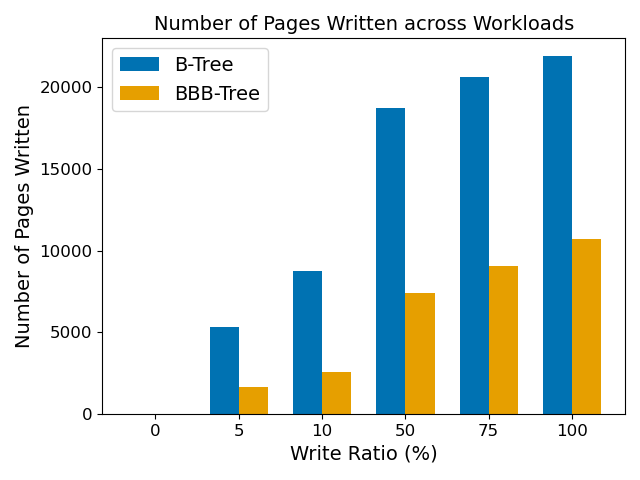
\includegraphics[width=\textwidth]{figures/evaluation/pageviews_write_ratios.png}
    \caption{Page Writes per workload.}
    \label{fig:write-ratios-page-writes}
  \end{subfigure}
  \hfill
  \begin{subfigure}[t]{0.49\textwidth}
    \centering
    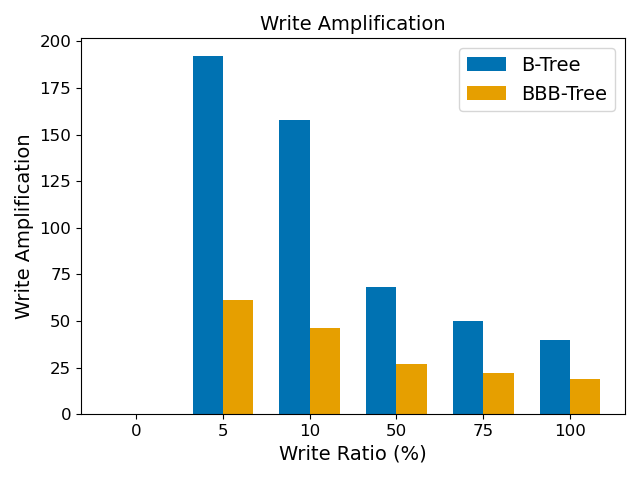
\includegraphics[width=\textwidth]{figures/evaluation/pageviews_write_ratios_wa.png}
    \caption{Write Amplification per workload.}
    \label{fig:write-ratios-wa}
  \end{subfigure}
  \caption{Page Writes and Write Amplification of the B-Tree and BBB-Tree with different write/read ratios in the workload. Without updates we have no page writes and therefore no write amplification. While page writes increase with more updates, write amplification decreases, as more changes happen in the same pages. The BBB-Tree can reduce write amplification significantly across all workloads.}  
  \label{fig:write-ratios}
\end{figure}

\subsection{Space Utilization}
\label{sec:space_overhead}
To track changes we need to store additional metadata in the B-Tree nodes.
This introduces a fixed overhead per B-Tree node.

\inlinesection{Tracking Modified Entries.}
Firstly, we store the state of each entry in the B-Tree node to track whether it has been modified or not.
We inject this information into the slot of each entry.
As mentioned in \autoref{chap:implementation}, we can use 2 bits to encode each state (Unchanged, Inserted, Updated, Deleted).
Since the slot data layout is critical to maximize fanout, we hide this information in the existing slot structure.
We use the two most significant bits of the offset to store the state.

\inlinesection{Tracking Degree of Change of Nodes.}
Secondly, we track the degree of change for each node.
To that end we store a counter in each B-Tree node that tracks the approximate number of bytes that have been modified since the last write to disk.
This counter is used to determine whether the write threshold has been reached and the node needs to be written to disk.
We use a 16-bit unsigned integer for this counter, which allows us to track changes up to 65535 bytes.
This is sufficient for our use case, as we can track changes up to 100\% of a 16 KB page.
More realistically though, we do not want to track changes beyond 50\% of a page, therefore we could even track larger page sizes with this counter.

This means that our implementation introduces a fixed overhead of 2 B per node.
However, this does not affect the fanout of the index significantly.
In some scenarios, it does not affect the fanout at all.
For example, when we store entries of fixed size 16 B (8 B key, 8 B value) on 4 KB pages as we do in our previous benchmarks.
On a leaf node, each entry requires 24 B, a slot of 8 B (4 B offset, 2 B key size, 2 B value size) and the data of 16 B (8 B key, 8 B value).
Therefore, our B-Tree leaf nodes can hold 170 entries on a 4 KB page.
With a header of 12 B, a full leaf node occupies $12 B + 170 * 24 B = 4092 B$.
With the additional overhead of 2 B per node, $ 4092 B + 2 B = 4094 B < 4096 B$, we can still fit the same amount of entries on a page.
The same applies to inner nodes.
In this scenario, we do not lose any fanout due to the additional overhead.
However, in other scenarios we might lose one entry per node due to the additional overhead.
With a 4 KB page and 170 entries per node, loosing one entry means a loss of \textasciitilde0.6\% in fanout.

% TODO: Maybe also add a section of the space overhead of saving deltas and its data layout.

\subsection{In-Memory Overhead}
To analyze the memory overhead of tracking changes on the pages in memory, we run the mixed Wikipedia Pageviews workload purely in memory, once on a B-Tree with tracking enabled and once on a B-Tree without tracking.
The B-Tree without tracking does not have a Delta Tree attached, so we can see the pure overhead of tracking changes in the B-Tree nodes.
We fixate the buffer pool size to 600 pages to ensure that the whole index fits in memory.
This way we can look at the pure memory overhead without the influence of page swaps.
The results are shown in \autoref{tab:tracking-overhead}.
We see that the overhead of tracking changes in memory is negligible.

\begin{table}[ht]
\centering
\begin{tabular}{l|l}
\toprule
\textbf{Index Type} & Time \\
\midrule
\textbf{B-Tree without Tracking}  & 13.54 ms \\
\textbf{B-Tree with Tracking}  & 13.55 ms (+0.07\%) \\
\bottomrule
\end{tabular}
\caption{Time to insert the Wikipedia Pageviews workload on an empty B-Tree with and without tracking changes. The buffer manager fits the whole index in memory. The memory overhead of tracking changes is negligible.}
\label{tab:tracking-overhead}
\end{table}

\subsection{Read Amplification}
Looking at write amplification does not give the full picture of the performance of the BBB-Tree.
We need to consider the read amplification that we introduce as well.
For the purpose of this analysis, we define read amplification as the ratio of page reads we add compared to the traditional B-Tree.

We introduce read amplification in the following way:
Everytime we load a B-Tree page from disk, we have to check the Delta Tree for any changes that need to be applied.
Everytime we unload a B-Tree's dirty page, we either delete its delta from the Delta Tree (if the page is written to disk) or insert/update its delta in the Delta Tree (if the page is not written to disk).
Since we have less space in memory for B-Tree pages, we have to swap B-Tree pages more often.
Therefore, we have more operations on the Delta Tree.
Any of the nodes in the Delta Tree that we access might not be in memory, leading to additional page reads.

We have illustrated the page traffic in the buffer pool in \autoref{fig:buffer-traffic} for a mixed workload with 5\% updates.

The Delta Tree is \textasciitilde6\% of the size of the B-Tree (30 nodes vs. 502 nodes).
We limited the buffer pool to 200 pages.
As expected, the BBB-Tree has more total buffer accesses due to the Delta Tree.
The accesses by the B-Tree are the same for both indices, since they process the same workload.
Since the buffer pool is shared with the Delta Tree, the BBB-Tree has slightly less space to cache B-Tree pages, leading to slightly more buffer misses for B-Tree accesses.
Each B-Tree page read is amplified further by the additional accesses to the Delta Tree that each B-Tree page read causes.
As we can see, most accesses to the Delta Tree are already buffered, since the Delta Tree is small in both cases.
While the additional buffer misses seem small compared to the buffer hits, they are significant in absolute terms.
After all, every buffer miss translates into an \ac{IO} operation to read the page from disk and potentially another \ac{IO} operation to write a dirty page back to disk to make space in the buffer pool.

For read amplification to remain low, we need to be able to cache the Delta Tree effectively in memory.
If we can cache most of the Delta Tree pages in memory, we only introduce a small number of additional page reads.
Therefore, the size of the Delta Tree compared to the available memory is critical to keep read amplification low.
This is another reason to keep the write threshold small, as it keeps the Delta Tree small.
We can analyze the maximum size of the Delta Tree given the write threshold and the size of the B-Tree:
Every node in the B-Tree can produce deltas of the maximum size of $write\_threshold * page\_size$ that need to be stored in the Delta Tree.
Therefore, the maximum size of all deltas is $write\_threshold * page\_size * num\_btree\_nodes$, which the Delta Tree has to store.
Since the Delta Tree has the same page size as the B-Tree, we can calculate the maximum number of leaf nodes in the Delta Tree (we neglect the space overhead of storing deltas in nodes for simplicity here):
$$num\_delta\_leaf\_nodes =  write\_threshold * num\_btree\_nodes$$
With a write threshold of 5\% for example, the number of leaf nodes in the Delta Tree are around 5\% of the total nodes of the B-Tree.
If 1\% of the B-Tree nodes are inner nodes, we can assume that that inner nodes are always cached in memory.
Therefore, we can simplify the number of Delta Tree nodes to:
$$num\_delta\_leaf\_nodes =  write\_threshold * num\_btree\_leaf\_nodes$$

We have shown in a previous section that the write threshold should be kept small to maximize write amplification reduction.
Also, we have seen that the amount of change per page usually remains small between page writes, leading to small deltas even with higher write thresholds.
Therefore, we can keep the Delta Tree small compared to the B-Tree, allowing us to cache it effectively in memory and keep read amplification low.

\begin{figure}[htbp]
  \centering
  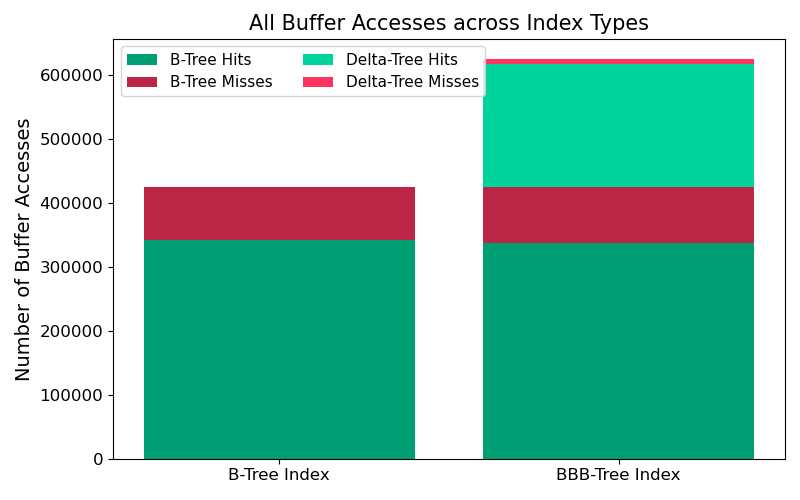
\includegraphics[width=0.7\textwidth]{figures/evaluation/pageviews_buffer_accesses_mixed.png}
  \caption{Total Buffer Accesses per index, separated into B-Tree accesses and Delta Tree accesses and their respective buffer hits and misses. Both indices have the same amount of B-Tree accesses (since they process the same workload), however the BBB-Tree causes more buffer misses since it also buffers the Delta Tree. This benchmark runs with a buffer pool of 200 pages, a page size of 4 KB, and a write threshold of 5\%. The B-Tree has 502 nodes.} 
  \label{fig:buffer-traffic}
\end{figure}

To repeat, while we can cache most of the Delta Tree in memory, we still introduce some additional page reads due to the introduced page overhead.
We have illustrated the total \ac{IO} operations, separated in reads and writes, in \autoref{fig:total-io} for different update ratios in the workload.
We can see that the that the baseline B-Tree performs the same amount of reads across all workloads, since the workload size and the index size remain the same.
We only change the amount of updates in the workload, which affects the amount of writes.
In contrast, the BBB-Tree perform more reads the higher the update threshold is, due to the read amplification we introduce.
However, the more writes we have in the workload, the more writes we can save with the BBB-Tree.
The read amplification is up to \textasciitilde33\%, while the write reduction is up to \textasciitilde62\%.

\begin{figure}[htbp]
  \centering
  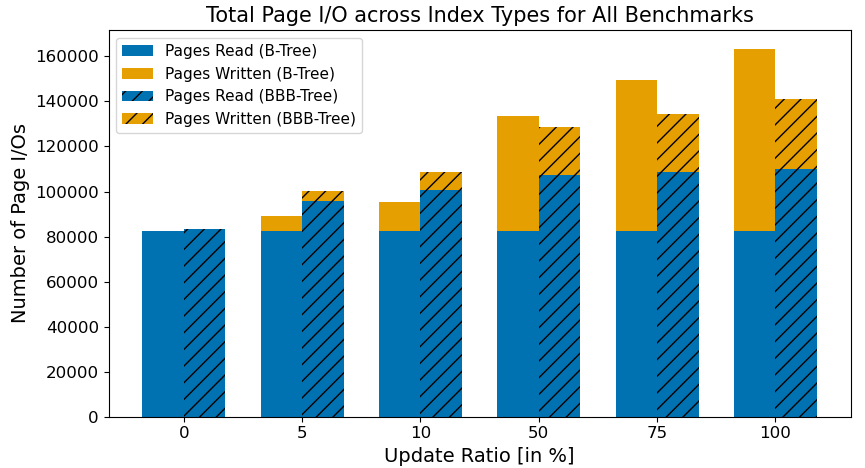
\includegraphics[width=0.7\textwidth]{figures/evaluation/pageviews_total_io_across_update_ratios.png}
    \caption{Total \ac{IO} operations per index, separated into reads and writes with different update ratios in the workload. When we introduce more page reads than we save page writes, we have more total \ac{IO} operations. This benchmark runs with a buffer pool of 200 pages, a page size of 4 KB, and a write threshold of 5\%. The B-Tree has 502 nodes.}
  \label{fig:total-io}
\end{figure}

These findings show that the BBB-Tree is not always beneficial in every scenario.
While we can reduce write amplification significantly, we introduce read amplification in the process.
Only in workloads where we have enough writes to compensate for the additional reads, we can achieve a net reduction in \ac{IO} operations.

We can express this trade-off in a payoff condition for our method.
Consider a workload consisting of $reads$ read operations and $writes$ write operations.
The proposed method amplifies reads by a fraction $read\_amplification$ (expressed as a percentage)  
and reduces writes by a fraction $write\_reduction$ (also in percent).

\begin{equation}
\frac{reads}{writes} < \frac{write\_reduction}{read\_amplification}
\label{eq:ratio_condition}
\end{equation}

For the case $c_w = c_r$ and the empirical values
$read\_amplification = 33\%$ and $write\_reduction = 62\%$ from the insert workload,  
Equation~\ref{eq:ratio_condition_costs} simplifies to:
\begin{equation}
\frac{reads}{writes} < \frac{62}{33} \approx 1.88
\end{equation}

Hence, the method pays off when the workload exhibits fewer than approximately $1.88$ read operations per write.
For example, in a workload where most pages are written to after being read from disk, we have one read per write most of the time $< 1.88$.
This is the pattern we see in the insert workload for example, building the index from scratch.
Also in update-heavy workloads, we can see such patterns.
For example in the 50\% update workload shown in \autoref{fig:total-io}, we have about 1.6 reads per write, so about 60\% of all read pages are written to before being evicted.
Since $1.6 < 1.88$, we reach a net reduction in \ac{IO} operations.
A scenario where our method performs very well. 

Depending on the underlying hardware, read and write operations can have different costs.
In a setting where random writes are significantly more expensive than random reads, as on the M1 Pro's SSD with 512 GB, we could see faster runs in the BBB-Tree even in scenarios where we have more total \ac{IO} operations due to a high fraction of read operations but less write operations.
However, some SSDs can be faster in writing than reading.
We can extend this condition to account for different costs of read and write operations.
Let $c_r$ and $c_w$ denote the cost per read and per write, respectively.  

% TODO: Maybe cite: https://www.reddit.com/r/mac/comments/1gvovdt/the_ultimate_guide_to_mac_ssd_speeds/#lightbox

\begin{equation}
\frac{reads}{writes} < \frac{c_w}{c_r} \cdot
\frac{write\_reduction}{read\_amplification}
\label{eq:ratio_condition_costs}
\end{equation}

To summarize, the BBB-Tree is beneficial in workloads where the majority of pages are written to after being read from disk, i.e. workloads with a low read-to-write ratio.
To keep read amplification low, we need to be able to cache the Delta Tree effectively in memory.

% Mixed workload, 400 pages in buffer, varying Update Ratio:
% - We consistently have 10\% more total IO.
% - When we lookup only, we have 1\% more IO.
% - We get up to 50\% more page misses on B-Tree pages even though the Delta Tree has only 59 nodes at max (100\% updates).
% - Delta Tree is up to 59 nodes.
% - We amplify reads more with 75\% updates.

% Mixed workload, 5\% udpates, varying Buffer Size:
% - We always have about 10\% more total IO. 

% Mixed workload, 5\% updates, 400 Buffer Size, varying Write Threshold:
% - with 0\% write threshold, we have 1\% more total IO, delta tree is 1 node
% - with 1\% write threshold, we have 4\% more total IO, delta tree is 16 nodes
% - with 5\% write threshold, we have 10\% more total IO, delta tree is 32 nodes
% - Why do we have so many delta nodes here? the insert workload operates on the same number of b-tree nodes but generates 19 delta nodes only.
% -> because more nodes produce small deltas in udpates between page swaps. In insertion more change than 5\% happens for most pages.

% Insert workload, varying Buffer Size:
% - With a buffer pool size of 400 we have 13\% less total IO
% - With a buffer pool size of 300 we have 20\% less total IO
% - With a buffer pool size of 200 we have 23\% less total IO
% - With a buffer pool size of 100 we have 17\% less total IO
% - We have enough page writes and less page reads -> net gain
% - Buffer Size does not really matter. We linearly have more/less total IO with smaller/larger buffer sizes.

% Insert workload, varying Write Threshold:
% - With no write threshold, we have 0.37\% more total IO
% - With a write threshold of 1\%, we have 12\% less total IO
% - With a write threshold of 5\%, we have 23\% less total IO
% - With a write threshold of 10\%, we have 17\% less total IO
% - With a write threshold of 15\%, we have 8\% less total IO
% - The higher the write threshold, the more page reads we have -> less net gain.

% We are not good in a scenario with very limited memory, as we constantly swap pages in and out of the buffer pool to perform operations on both trees.
% With more memory, we can cache the Delta Tree pages better, reducing read amplification.
% With too much memory, we amplify the reads too much because the B-Tree pages are mostly in memory already, where the Delta Tree hurts more.
% TODO: Show this in a figure.

\subsection*{Variable-Sized Entries}
To analyze the effect of variable-sized entries, we run the same Wikipedia Pageviews workload, but this time with the variable-sized \texttt{page\_title} as key.
As expected, the index size increases due to the larger average key size of \textasciitilde 20.5 B compared to the fixed size keys of 8 B.
We observed that the B-Tree has 757 nodes with variable-sized keys compared to 502 nodes with integer keys.
To remove the influence of different index sizes, and therefore more pages, we run the benchmarks with a buffer pool that fits \textasciitilde40\% of the B-Tree in memory respectively (300 pages for fixed-sized keys, 200 pages for variable-sized keys).
We run the same workload with 100\% insertions.
The results are shown in \autoref{fig:total-io-variable-size}.

\begin{figure}[htbp]
  \centering
  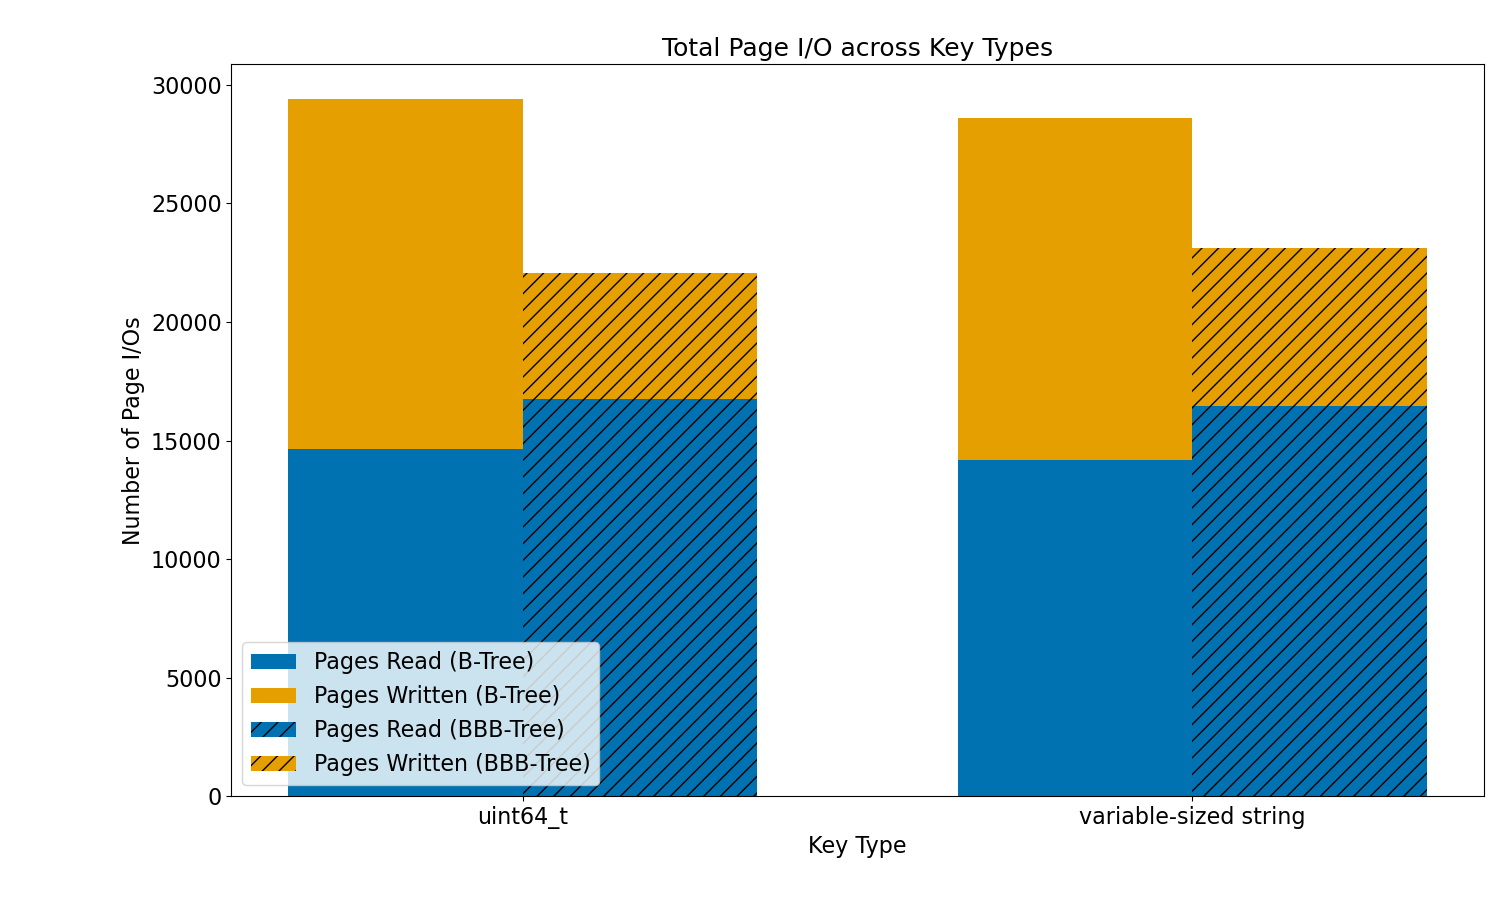
\includegraphics[width=0.9\textwidth]{figures/evaluation/pageviews_total_io_variable_size.png}
  \caption{Total \ac{IO} operations per index, separated into reads and writes with 100\% insertions of variable-sized string keys and fixed-sized integer keys. The buffer pool fits \textasciitilde40\% of the B-Tree in memory, the page size is 4 KB and the write threshold is 5\%. While we can reduce total \ac{IO} operations in both cases, the write reduction is smaller with variable-sized keys.}
  \label{fig:total-io-variable-size}
\end{figure}

With the different buffer sizes we achieve similar page reads and writes for the baseline B-Trees.
However, with variable-sized keys, the BBB-Tree achieves a smaller reduction in page writes compared to fixed-sized keys.
With variable-sized keys, we can reduce page writes by \textasciitilde56\% compared to \textasciitilde64\% with fixed-sized keys.
The reason is that with variable-sized keys, we have more B-Tree nodes with more than 5\% eviction time as shown in \autoref{tab:modification-degree-variable-size}.
Therefore, we buffer fewer page writes in the Delta Tree, leading to a smaller write reduction.

While a conclusion could be that variable sized keys require a larger write threshold to achieve similar write reductions, we could not confirm this hypothesis with our experiments.
Just as with fixed-sized keys, we see diminishing returns with larger write thresholds, because the Delta Tree becomes larger, leading to higher read amplification.

\begin{table}[ht]
\centering
\begin{tabular}{l|cc}
   \toprule
    & \multicolumn{2}{c}{\textbf{Num. Pages}} \\
    \cmidrule(lr){2-3}
    \textbf{Modified} & \textbf{Fixed-Size Keys} & \textbf{Variable-Size Keys} \\
    \midrule
    0-5     & 12487 & 11013 \\
    5-10    & 2470  & 3303  \\
    10-15   & 64    & 180   \\
    15-20   & 5     & 26    \\
    20-25   & 1     & 4     \\
    25-30   & 0     & 2     \\
    30-35   & 0     & 0     \\
    35-40   & 0     & 1     \\
    40-45   & 0     & 10    \\
    45-50   & 104   & 239   \\
    50-55   & 446   & 477   \\
    55-60   & 59    & 139   \\
    60-65   & 15    & 43    \\
    65-70   & 13    & 23    \\
    70-75   & 11    & 19    \\
    75-80   & 5     & 16    \\
    80-85   & 2     & 13    \\
    85-90   & 7     & 9     \\
    90-95   & 6     & 11    \\
    95-100  & 9     & 13    \\
    >=100   & 109   & 163   \\
    \midrule
    Total Evictions & 15813 & 15705 \\
\bottomrule
\end{tabular}
\caption{Distribution of B-Tree pages by their modification degree (percentage intervals) when being evicted with a Write Threshold of 5\% for fixed-sized keys and variable-sized keys in a workload with 100\% insertions. While both have similar number of page evictions, the variable-sized keys have more variance in the modification degree and less pages with a degree of change below the write threshold of 5\%.}
\label{tab:modification-degree-variable-size}
\end{table}


Both Delta Trees are \textasciitilde3.8\% of the size of their respective B-Trees.
Even though we might have larger deltas with variable-sized keys, we decide to produce a delta based on the percentage of the page size that has changed.
The amount of bytes that can be accumulated in a delta are the same in both cases, since both have a write threshold of 5\% on 4 KB pages.
Therefore, we do not increase the size of the Delta Tree with variable-sized keys.

% \subsection*{Different Page Sizes}

%TODO: Compare performance with sequential updates vs random updates.
